\appendix
\section{Appendix MPC-L} \label{AppendixA}
As introduced in Section \ref{subsection:failed_tests}, during the single static obstacle avoidance testing phase, we have encountered some issues regarding the validation of the sixth requirement on the speed range specified in Section \ref{System_Requirements}. In particular, after verifying that the MPC we were developing was unable to perform well at low speeds (under 40 $km/h$), we have decided to split the main problem into two sub-problems consisting of two different speed ranges which would be managed by two different MPCs.
This choice has allowed us to continue the validation relative to MPC-H, which is the one managing high speeds (from 40 to 100 $km/h$), avoiding going back to modify the parameters of the controller to find an optimal solution (if it exists) working in the whole range of speeds.

This Appendix, instead, is dedicated to the development of the MPC-L, which manages the speeds ranging from 10 to 40 $km/h$. After validating the MPC-H, we have come back to its parameters definition and then we have set up a testing procedure where we have applied several different combinations acting on prediction horizon, sample time, and output variables weights of the cost function, aimed to find an appropriate solution.
The test setup and outcomes can be found in the Documentation folder of the repository\footnote{The ``MPC-L-Test\_Report001",\space``MPC-L-Test\_Report002",\space``MPC-L-Test\_Report0005", and ``MPC-L-Test\_Specification\_Report" files generated by Simulink Test are included in the Documentation/Test Reports/MPC-L\_Test\_Reports/ file path.}.\\
Thanks to this iterations, we have found a suitable set of parameters working at 20 $km/h$, that is reported in the following table:
\begin{table}[H]
\centering
\begin{tabular}{|l|l|}
\hline
Prediction Horizon & 10               \\ \hline
Sample Time        & 0.02             \\ \hline
WOV                & {[}30 30 8 30{]} \\ \hline
\end{tabular}
\caption{Best configuration found for MPC-L}
\label{tab:MPC_L_Config}
\end{table}
With the configuration reported in Table \ref{tab:MPC_L_Config}, we have run the test for the static obstacle avoidance in the scenarios already used in Section \ref{chap:static_obstacle_avoidance_tests}, setting a constant speed of 20 $km/h$. The results of this test, as usual, are reported in the Documentation folder\footnote{The ``MPC-L\_Static\_Obstacle\_Avoidance-Test\_Report" and ``MPC-L\_Static\_Obstacle\_Avoidance-Test\_Specification\_Report" files generated by Simulink Test are included in the Documentation/Test Reports/MPC-L\_Test\_Reports/ file path.}.
Even if this configuration seems to work pretty well on most of the scenarios, we have still found that in some situations the controller loses stability and starts oscillating, as shown in Figure \ref{fig:mpc_l_test}.

\begin{figure}[H]
    \centering
    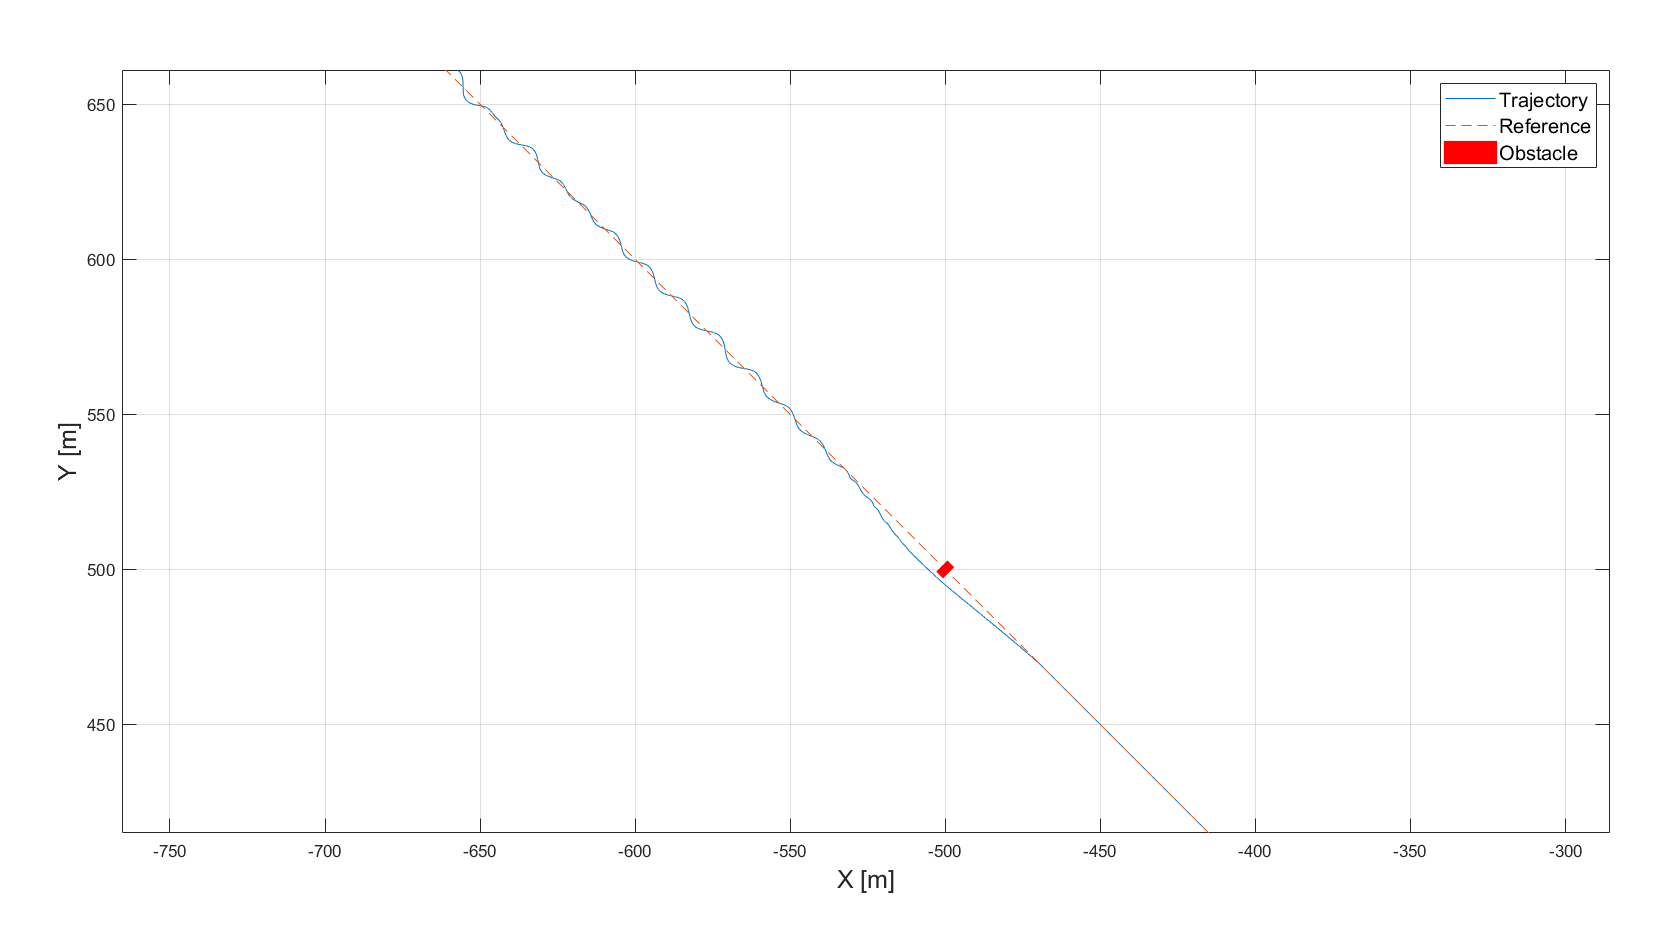
\includegraphics[width=\textwidth,keepaspectratio]{Figures/mpc_l_test_169.png}
    \caption{Output Trajectory of the Vehicle with MPC-L controller in 135° scenario}
    \label{fig:mpc_l_test}
    \end{figure}
    
   
In order to get the best out of this controller, further tuning is required but we have decided to stop here because this goes beyond the didactic purpose of this particular project. 